% UCL Thesis LaTeX Template
%  (c) Ian Kirker, 2014
% 
% This is a template/skeleton for PhD/MPhil/MRes theses.
%
% It uses a rather split-up file structure because this tends to
%  work well for large, complex documents.
% We suggest using one file per chapter, but you may wish to use more
%  or fewer separate files than that.
% We've also separated out various bits of configuration into their
%  own files, to keep everything neat.
% Note that the \input command just streams in whatever file you give
%  it, while the \include command adds a page break, and does some
%  extra organisation to make compilation faster. Note that you can't
%  use \include inside an \include-d file.
% We suggest using \input for settings and configuration files that
%  you always want to use, and \include for each section of content.
% If you do that, it also means you can use the \includeonly statement
%  to only compile up the section you're currently interested in.
% You might also want to put figures into their own files to be \input.

% For more information on \input and \include, see:
%  http://tex.stackexchange.com/questions/246/when-should-i-use-input-vs-include

% Formatting rules for theses are here: 
%  http://www.ucl.ac.uk/current-students/research_degrees/thesis_formatting
% Binding and submitting guidelines are here:
%  http://www.ucl.ac.uk/current-students/research_degrees/thesis_binding_submission

% This package goes first and foremost, because it checks all 
%  your syntax for mistakes and some old-fashioned LaTeX commands.
% Note that normally you should load your documentclass before 
%  packages, because some packages change behaviour based on
%  your document settings.
% Also, for those confused by the RequirePackage here vs usepackage
%  elsewhere, usepackage cannot be used before the documentclass
%  command, while RequirePackage can. That's the only functional
%  difference.
\RequirePackage[l2tabu, orthodox]{nag}

% ------ Main document class specification ------
% The draft option here prevents images being inserted,
%  and adds chunky black bars to boxes that are exceeding 
%  the page width (to show that they are).
% The oneside option can optionally be replaced by twoside if
%  you intend to print double-sided. Note that this is
%  *specifically permitted* by the UCL thesis formatting
%  guidelines.
%
% Valid options in terms of type are:
%  msc
%  phd
%  mres
%  mphil
%\documentclass[12pt,phd,draft,a4paper,oneside]{ucl_thesis}
\documentclass[12pt,msc,a4paper,oneside]{ucl_thesis}

% Package configuration:
%  LaTeX uses "packages" to add extra commands and features.
%  There are quite a few useful ones, so we've put them in a 
%   separate file.
% -------- Packages --------

% This package just gives you a quick way to dump in some sample text.
% You can remove it -- it's just here for the examples.
\usepackage{blindtext}

% This package means empty pages (pages with no text) won't get stuff
%  like chapter names at the top of the page. It's mostly cosmetic.
\usepackage{emptypage}

% The graphicx package adds the \includegraphics command,
%  which is your basic command for adding a picture.
\usepackage{graphicx}

% This command is provided by the graphicx package, and 
%  controls the default dpi resolution of images you use.
%  72 is the default, but 300 is more normal, and 600 is
%  as good as you can expect to be able to get on normal paper.
\pdfimageresolution=300


% The float package improves LaTeX's handling of floats,
%  and also adds the option to *force* LaTeX to put the float
%  HERE, with the [H] option to the float environment.
\usepackage{float}

% The amsmath package enhances the various ways of including
%  maths, including adding the align environment for aligned
%  equations.
\usepackage{amsmath}

% Use these two packages together -- they define symbols
%  for e.g. units that you can use in both text and math mode.
\usepackage{gensymb}
\usepackage{textcomp}
% You may also want the units package for making little
%  fractions for unit specifications.
%\usepackage{units}


% The setspace package lets you use 1.5-sized or double line spacing.
\usepackage{setspace}
\setstretch{1.5}

% That just does body text -- if you want to expand *everything*,
%  including footnotes and tables, use this instead:
%\renewcommand{\baselinestretch}{1.5}


% PGFPlots is either a really clunky or really good way to add graphs
%  into your document, depending on your point of view.
% There's waaaaay too much information on using this to cover here,
%  so, you might want to start here:
%   http://pgfplots.sourceforge.net/
%  or here:
%   http://pgfplots.sourceforge.net/pgfplots.pdf
%\usepackage{pgfplots}
%\pgfplotsset{compat=1.3} % <- this fixed axis labels in the version I was using

% PGFPlotsTable can help you make tables a little more easily than
%  usual in LaTeX.
% If you're going to have to paste data in a lot, I'd suggest using it.
%  You might want to start with the manual, here:
%  http://pgfplots.sourceforge.net/pgfplotstable.pdf
%\usepackage{pgfplotstable}

% These settings are also recommended for using with pgfplotstable.
%\pgfplotstableset{
%	% these columns/<colname>/.style={<options>} things define a style
%	% which applies to <colname> only.
%	empty cells with={--}, % replace empty cells with '--'
%	every head row/.style={before row=\toprule,after row=\midrule},
%	every last row/.style={after row=\bottomrule}
%}


% The mhchem package provides chemistry formula typesetting commands
%  e.g. \ce{H2O}
%\usepackage[version=3]{mhchem}

% And the chemfig package gives a weird command for adding Lewis 
%  diagrams, for e.g. organic molecules
%\usepackage{chemfig}

% The linenumbers command from the lineno package adds line numbers
%  alongside your text that can be useful for discussing edits 
%  in drafts.
% Remove or comment out the command for proper versions.
%\usepackage[modulo]{lineno}
% \linenumbers 


% Alternatively, you can use the ifdraft package to let you add
%  commands that will only be used in draft versions
%\usepackage{ifdraft}

% For example, the following adds a watermark if the draft mode is on.
%\ifdraft{
%  \usepackage{draftwatermark}
%  \SetWatermarkText{\shortstack{\textsc{Draft Mode}\\ \strut \\ \strut \\ \strut}}
%  \SetWatermarkScale{0.5}
%  \SetWatermarkAngle{90}
%}


% The multirow package adds the option to make cells span 
%  rows in tables.
\usepackage{multirow}


% Subfig allows you to create figures within figures, to, for example,
%  make a single figure with 4 individually labeled and referenceable
%  sub-figures.
% It's quite fiddly to use, so check the documentation.
%\usepackage{subfig}

% The natbib package allows book-type citations commonly used in
%  longer works, and less commonly in science articles (IME).
% e.g. (Saucer et al., 1993) rather than [1]
% More details are here: http://merkel.zoneo.net/Latex/natbib.php
%\usepackage{natbib}

% The bibentry package (along with the \nobibliography* command)
%  allows putting full reference lines inline.
%  See: 
%   http://tex.stackexchange.com/questions/2905/how-can-i-list-references-from-bibtex-file-in-line-with-commentary
\usepackage{bibentry} 

% The isorot package allows you to put things sideways 
%  (or indeed, at any angle) on a page.
% This can be useful for wide graphs or other figures.
%\usepackage{isorot}

% The caption package adds more options for caption formatting.
% This set-up makes hanging labels, makes the caption text smaller
%  than the body text, and makes the label bold.
% Highly recommended.
\usepackage[format=hang,font=small,labelfont=bf]{caption}

% If you're getting into defining your own commands, you might want
%  to check out the etoolbox package -- it defines a few commands
%  that can make it easier to make commands robust.
\usepackage{etoolbox}


% Sets up links within your document, for e.g. contents page entries
%  and references, and also PDF metadata.
% You should edit this!
%%
%% This file uses the hyperref package to make your thesis have metadata embedded in the PDF, 
%%  and also adds links to be able to click on references and contents page entries to go to 
%%  the pages.
%%

% Some hacks are necessary to make bibentry and hyperref play nicely.
% See: http://tex.stackexchange.com/questions/65348/clash-between-bibentry-and-hyperref-with-bibstyle-elsart-harv
\usepackage{bibentry}
\makeatletter\let\saved@bibitem\@bibitem\makeatother
\usepackage[pdftex,hidelinks]{hyperref}
\makeatletter\let\@bibitem\saved@bibitem\makeatother
\makeatletter
\AtBeginDocument{
    \hypersetup{
        pdfsubject={Network Science, Network Analysis, Community Detection},
        pdfkeywords={network science, network analysis, community detection},
        pdfauthor={Sergiu Tripon},
        pdftitle={Detecting community structure in EPSRC Research Grant-based Networks},
    }
}
\makeatother
    


% And then some settings in separate files.
% These settings are from:
%  http://mintaka.sdsu.edu/GF/bibliog/latex/floats.html

% They give LaTeX more options on where to put your figures, and may
%  mean that fewer of your figures end up at the tops of pages far
%  away from the thing they're related to.

% Alters some LaTeX defaults for better treatment of figures:
% See p.105 of "TeX Unbound" for suggested values.
% See pp. 199-200 of Lamport's "LaTeX" book for details.

%   General parameters, for ALL pages:
\renewcommand{\topfraction}{0.9}	% max fraction of floats at top
\renewcommand{\bottomfraction}{0.8}	% max fraction of floats at bottom

%   Parameters for TEXT pages (not float pages):
\setcounter{topnumber}{2}
\setcounter{bottomnumber}{2}
\setcounter{totalnumber}{4}     % 2 may work better
\setcounter{dbltopnumber}{2}    % for 2-column pages
\renewcommand{\dbltopfraction}{0.9}	% fit big float above 2-col. text
\renewcommand{\textfraction}{0.07}	% allow minimal text w. figs

%   Parameters for FLOAT pages (not text pages):
\renewcommand{\floatpagefraction}{0.7}	% require fuller float pages
% N.B.: floatpagefraction MUST be less than topfraction !!
\renewcommand{\dblfloatpagefraction}{0.7}	% require fuller float pages

% remember to use [htp] or [htpb] for placement,
% e.g. 
%  \begin{figure}[htp]
%   ...
%  \end{figure} % For things like figures and tables
\bibliographystyle{unsrt}   % For bibliographies

% Title Settings
\setcounter{secnumdepth}{3}
\setcounter{tocdepth}{3}
\title{Detecting community structure in EPSRC Research Grant-based Networks}
\author{Sergiu Tripon}
\department{Department of Computer Science}

\begin{document}

\nobibliography*
% This is a dumb trick that works with the bibentry package to let
%  you put bibliography entries whereever you like.
% I used this to put references to papers a chapter's work was 
%  published in at the end of that chapter.
% For more information, see: http://stefaanlippens.net/bibentry

% If you haven't finished making your full BibTex file yet, you
%  might find this useful -- it'll just replace all your
%  citations with little superscript notes.
% Uncomment to use.
%\renewcommand{\cite}[1]{\emph{\textsuperscript{[#1]}}}

% At last, content! Remember filenames are case-sensitive and 
%  *must not* include spaces.
\maketitle
\makedeclaration

\begin{abstract} % 300 word limit
My research is about stuff.

It begins with a study of some stuff, and then some other stuff and things.

There is a 300-word limit on your abstract.
\end{abstract}

\begin{acknowledgements}
Acknowledge all the things!
\end{acknowledgements}

\setcounter{tocdepth}{2} 
% Setting this higher means you get contents entries for
%  more minor section headers.

\tableofcontents
\listoffigures
\listoftables

\chapter{\textsc{Introduction}}
\label{chapterlabel1}

Every day, humans produce valuable intelligence which can be used further in significant areas such as analysis, prediction, decision-making and many others. For example, when a user repeatedly watches tv series or films on Netflix, without realising, they provide Netflix with invaluable data in regards to their preferences including genre, type and language. Their user account also provides useful information such as gender, age, when and how often they use Netflix, the platform they access Netflix from and much more. This information can be analysed by Netflix as part of a research project in order to gather compelling insights into the data. The results of this research project can then have an impact in decision-making. For example, when deciding which series Netflix should add next to the platform based on user demand of a specific genre. It can also be used to improve the prediction of their recommender system. However, not everyone makes use of the gathered intelligence, and often, the opportunity to take advantage of it, goes missing.

One of the institutions that posses such important and substantial intelligence data is EPSRC. Currently, EPSRC holds a significant number of topics used by researchers to classify research grants when making a proposal. Furthermore, EPSRC are facing a difficult task in determining how fine or coarse the topics should be defined. Subsequently, they are also uncertain on how this could be achieved, once the definition is determined.

This research project primarily seeks to cluster research topics into research areas using grant data collected from EPSRC. A secondary objective involves the clustering of researchers into research communities. The project aims to achieve this through applying a novel approach to a real world problem, involving graph theory, network science, the concept of modularity and community detection. Therefore, as much as the objectives are the clustering of topics and researchers, verifying whether this approach can be used to solve this kind of problems is also a crucial objective. It is expected that this approach will provide a cogent way to group topics in terms of similarity and aid decision making regarding their definition.

A number of different interpretations of the data collected from EPSRC were turned into \textit{Networks of Topics} and \textit{Researchers}. A further two different interpretations of each network were considered. Also, five different edge weight interpretations and eight community detection algorithms were considered. These amounts were refined to one optimal combination of edge weight interpretation and community detection algorithm, while the two different interpretations of each network were compared. Further details regarding the networks, edge weight interpretations and community detection algorithms are provided later in the thesis.

It was found that using the \textit{Topic network (Grants as edges)} produced a more rational topic clustering in comparison to the \textit{Researchers as edges} interpretation of it. In contrast, the \textit{Researcher network (Topics as edges)} network performed better than the \textit{Researcher network (Grants as edges)} when considering the researcher clustering. Furthermore, the edge weight normalized by the number of grants proved to be optimal. The results also showed that the Louvain method produced the most rational and well-defined clustering compared to the other community detection algorithms considered.

\section{Structure of this Thesis}

The remainder of this thesis is structured as follows. Chapter 2 provides an introduction to EPSRC and the problem addressed as well as concepts used throughout the project. Chapter 3 reviews the literature consulted during the project and highlights its contribution. The methodology followed throughout the project is described in Chapter 4. The results of the project are presented, compared and discussed in Chapter 5 and their evaluation is also documented. In Chapter 6, the work carried out throughout the project is summarised and concluded, and further potential work is recommended.

\iffalse
\section{Motivation and Scope}

\section{Scope}

Every day people produce some sort of useful and valuable intelligence, from booking a fight with easyJet to watching a movie on Netflix.

When using these services, people provide information regarding their preferences including their seat choice, or movie genre. After several uses, companies can make use of the intelligence gathered and improve the service experience through prediction. The intelligence can also be used in research.

However, a lot of the time, the intelligence goes unnoticed and the opportunity of making valuable use of it is missed.

This project aims to cluster research topics into research areas using current and historical grant data publicly provided by EPSRC.

EPSRC (Engineering and Physical Science Research Council) is the main UK government agency for funding research and training in engineering and the physical sciences \cite{epsrc_about_us}.

Recently during a talk, an EPSRC officer revealed the fact that there are a lot of complaints about the way research areas and researcher communities are defined within EPSRC. The officer stated that it was not clear how fine or coarse they should be divided, and that they should be constantly changed to reflect the funding and research trend.

EPSRC makes grant data available online through its Grants on the Web (GoW) service. Each grant record includes valuable information, from which various networks can be constructed and analysed including a topic and researcher-based network which this study focuses on.

This research project seeks to identify and analyse the community structure in the networks constructed using network analysis. Moreover, it aims to observe the data from a number of different perspectives. Firstly, the project analyses data from three different time periods: 1990-2000, 2000-2010 and current data. Secondly, the number and value of the research grants are incorporated as attributes to add a numerical and financial insight to the data. Correlations between the trends and community structure identified and other data factors may prove insightful.

I believe that this study will achieve its goals and produce valuable results. They will provide a deeper understanding of the community structure identified and how it can help decision-making in regards to the definition of topics and researcher communities within EPSRC. Furthermore, the time, numerical and financial elements will aid in providing answers and insights along the way.
\fi

\iffalse
\section{Research tasks}

This study has one specific area of research defined, the detection of community structure in the networks constructed from the collected grant data. Additionally, the study aims to analyse various other points of interest. Besides community detection, an extremely important breakthrough focuses on determining whether the community structures identified are reliable and their level of reliability. This also involves comparing them to other community structures identified in other projects with a similar theme.

Basic statistics of each network will also be computed and analysed  in order to gather insights into why the relationships within the networks are laid out the way they are. This will involve time comparison, as well as making use of other data attributes to help determine whether these attributes have an impact on the network's general or community structure. 

By combining the different areas of research identified, a number of research questions the project seeks to answer were compiled and are listed below:

\begin{enumerate}[itemsep=0cm]
    \item What are the significant network metrics of each network?
    \item Does each network hold a community structure?
    \item How large is the community structure identified in each network?
    \item Is there a similarity between the network community structure identified in this project compared to other research projects?
    \item Is the community structure identified in each network cogent?
    \item Do any interesting trends arise when comparing networks from different time periods?
    \item Does the number and value of research grants have an impact on the network's general structure and community structure?
\end{enumerate}
\fi

\iffalse
\section{Value}

Currently, the EPSRC Portfolio consists of 223 topics and 3175 grants are classified by one or more topics. The number of topics has increased by 15 since 2010 and 87 since 1990. Considering this growth, it means that defining research topics becomes increasingly difficult. As the number of topics enlarges, the number of complaints does too, as opinions on how topics should be defined differ significantly. In contrast, the analysis of grant data could be the answer to the problem, receiving a boost in value and potential.

This project aims to find an answer to this issue through the use of network analysis and community detection algorithms. At the moment, EPSRC provides a Visualising our Portfolio (VOP) service which allows users to visualise a number of networks based on research themes, areas, and organisations. However, VOP does not provide a visualisation of a topic-based network. Analysing a topic-based network automatically fills a gap which EPSRC doesn't cover and will potentially find compelling.

Initially, when a topic-based network is constructed, there is no division between topics, they are all treated the same. The only difference is their relationships to other topics and their attribute values. Let's assume that a task involves addressing a problem in regards to defining topics coarser or finer in a reliable way i.e. too many similar topics or not enough topics to cover the grants. Attempting to achieve the task by focusing on the full network will prove extremely difficult. Subsequently, a potential alternative could involve grouping similar topics manually, and then analysing each group separately. This would lower the difficulty level compared to the previous attempt, but will significantly increase the time it would take to complete the task.

However, if a technique employed computationally would be used to "slice" the network into a number of smaller clusters, the task would be complete in time and with more ease. This project uses network analysis and community detection methods optimal to the network in order to determine a its community structure. This brings various benefits and substantial value to the process of defining topics within EPSRC.

Firstly, the complainants will be pleased to hear that there is now a solution in place which addresses their grievances. This should subsequently have an impact on the number of future complaints received by the EPSRC. Secondly, EPSRC can take advantage of the results produced by this study to construct a topic and researcher-based network while also illustrating their community structure to accompany the other networks already built within the VOP service. Finally, as part of potential future work, the community detection algorithms used can be applied to the other networks in order to also detect their community structure and visualise it.
\fi

\iffalse
\section{Data, Algorithms and Tools}

EPSRC provides current and past data through its GoW service. Current data comprises of grant records categorised by research area and topic among other research entities, while past data consists of unclassified grant records. Each grant record holds various information including the researchers, topic classifications and value of the grant. However, it does not store information regarding the research area of a grant. This project only takes in consideration data from research grant and researcher records. Due to this lack of information, research area-based networks can only be constructed from current grant data. In contrast, the creation of research topic-based networks covering all time periods is possible. The Data section of the Methodology chapter provides further details on this matter.

Algorithms are used for two purposes within this project: to compute the network's statistics and detect its community structure. This study focuses on metrics such as the average degree, average weighted degree diameter, radius, density, modularity, average clustering coefficient and average path length. Moreover, a wide variety of community detection methods are considered including Infomap, Spinglass, Louvain, Label Propagation, Leading Eigenvector and Walktrap.

During this study, a number of tools are used for programming, analysis and visualisation purposes. Programming is done in Python and Bash using Jetbrains PyCharm IDE. Microsoft Excel is used for data validation. iGraph, NetworkX, Stanford SNAP aid the network analysis and the detection of community structure in the networks. The visualisation of the networks is created using Gephi, Graphistry and Adobe Photoshop.
\fi

\iffalse
\section{Results and Achievements}

The project set out a number of objectives and questions expected to be achieved or answered, at the end of this project. The achieved objectives represent the results and achievements of the project and are used to measure the project's success.

A number of community detection algorithms are applied to the networks and the underlying community structure is revealed. This provides understanding of how communities are formed from a funding perspective. It also offers a way to determine whether the current definition of research topics is too fine or too coarse and how to control it in the right direction.

Moreover, data spanning across 30 years is used to construct the networks, adding a significant temporal effect to analysis. It means networks from different time periods are compared and their differences explored. This will provide an indication of the impact that time has on the relationships and communities of networks.

Furthermore, number and value attributes are included in the data to allow the analysis of the network from a numerical and financial perspective. The number and value attributes represent the number of common entities and the value of the common entities, respectively. Correlations between the identified community structure and the attributes are investigated in order to bring further answers and insights to the analysis process.
\fi

\iffalse
\section{Self-assessment}
I believe that the outcomes of this study are both interesting and valuable. In particular, detecting community structure in networks was something new for me and led me to develop a growing interest in the subject.

Working on this project offered me the opportunity to find answers to real world issues through network analysis. The results of this study range from constructing a number of networks from external data to determining whether the networks hold a community structure and subsequently identifying it.

Three aspects that I found extremely interesting to analyse were the time, numerical and financial factors of the data. Comparing networks from different time periods provided interesting results that answer questions in regards to the transition of the network's general and community structure.

Additionally, observing networks from a numerical and financial standpoint led to insightful results providing answers to question regarding specific network behaviours.

Overall, gaining an understanding of how communities are structured within research networks was extremely engaging, as it answered questions in regards to how the definition of topics could be improved, which would remain unanswered without network analysis.
\fi
\chapter{Background}
\label{chapterlabel2}

\section{Network Science}

\blindtext

\section{Community Detection}

\blindtext

\section{EPSRC}

\blindtext
\chapter{\textsc{Literature Survey}}
\label{chapterlabel3}

The Background chapter introduced EPSRC and the problem addressed in this research project while also providing background to several concepts in network science, community detection algorithms and other forms of classification. This section presents the literature reviewed prior to commencing this project identify related works and determine whether studies with a similar focus as this one have already been completed.

\vspace*{1em}

\textbf{Community Structure on Wikipedia} \cite{wikipedia_community_structure} documents community structure thoroughly and provided a good starting point to the literature survey. The article describes the properties and application of community structures in networks. Moreover, it gives a detailed description of a significant number of community detection algorithms as well as several testing methods enabling the evaluation of the algorithms. The information on Wikipedia helped to gain a general understanding of the subject and identify the further direction of the survey.

\vspace*{1em}

\textbf{Community Detection and Mining in Social Media} \cite{community_detection_class} is a class taught by \textit{Lei Tang} (Yahoo! Labs) and \textit{Huan Liu} (Arizona State University) at Arizona State University. The class follows the teachings of a book with the same name \cite{tang2010community} published by \textit{Lei Tang} and \textit{Huan Liu} in 2010. The information from the class is available online in the form of PowerPoint presentations. Essentially, they provide a summary, highlighting the most important parts from the book. The class added the academic knowledge required to the literature survey while also expanding on the information gathered from Wikipedia in regards to community detection evaluation.

\vspace*{1em}

\textbf{Community structure in social and biological networks} \cite{girvan2002community} is a research paper authored by \textit{Michelle Girvan} and \textit{Mark EJ Newman} and published in 2002. The research paper introduces the community structure property, present in many networks. It defines the community structure of a network as network nodes linked together in densely connected clusters, between which there are only sparser connections.

Girvan and Newman also propose a method to detect communities in networks which is built based on the idea of centrality indices. The method is tested on both \textit{real-world} and \textit{computer-generated} networks whose community structure is both known and unknown. \textit{Real-world} networks used for testing include \textit{Zachary's Karate Club Study} and \textit{College Football}. The study used networks without a known community structure such as the \textit{Collaboration} and \textit{Food Web} networks. In the case of a known community structure, the authors found that the method performed well and identified the known community structure with high-sensitivity and reliability. Furthermore, in both cases of unknown community structure, the method still detected significant and informative community divisions.

This research paper was extremely beneficial as it provided further knowledge in the field of community detection as well as the concepts and methods required to complete this research project.

\vspace*{1em}

\textbf{Finding and evaluating community structure in networks}
\cite{newman2004finding} is another paper published in 2004 by \textit{Mark EJ Newman} and \textit{Michelle Girvan} and similar to their previous collaborative work, \textit{Community structure in social and biological networks}. In this publication, the authors propose a set of algorithms for identifying community structure in networks, which is defined as "natural divisions of network nodes into densely connected subgroups." Moreover, this paper represents the introduction of the community structure measure known as \textit{modularity}.

The proposed algorithms include shortest-path betweenness, resistor networks and random walks. A way to measure the strength of the community structure identified by the algorithms proposed is also introduced. The measure provides an objective metric for determining the number of communities a network should be divided into. Testing the algorithms on both \textit{computer-generated} and \textit{real-world networks}, \textit{Newman} and \textit{Girvan} demonstrate that the algorithms are extremely effective at identifying community structure.

The knowledge gained from this study was extremely helpful throughout the duration of this project. It explained how the algorithms proposed were built and how they work, while also providing examples of networks on which the algorithms were evaluated on. It also showed the progress of \textit{Newman} and \textit{Girvan} in the subject since their previous collaborative research effort.

\vspace*{1em}

\textbf{Topic oriented community detection of rating based social networks} is a study conducted by \textit{Reihanian et al.} \cite{reihanian2015topic} in 2015 focusing on community detection from the perspective of content analysis. Most community detection research chooses to focus only on the topological structure of the network. In a social network, for example, this is usually based on the number of communications among individuals. In contrast, this research paper aims to go further and explore and analyse the network's content flow.

The development process of the project commences by preprocessing and annotating topic labels and continues with the clustering of social objects and the creation of topic clusters. It concludes by applying a community detection algorithm to the produced topical clusters in order to identify the community structure within each cluster. Furthermore, a number of experiments are carried out on several data sets including \textit{Movielens 100k}, \textit{Book-Crossing}, \textit{CIAO}, \textit{MovieTweetings} and \textit{Movielens Latest}. It makes use of a performance metric, \textit{purity}, as defined by Zhao et al. \cite{zhao2012topic} which considers both topic and linkage structure. It identifies a maximum \textit{purity} value in each experiment as the topical clusters created in each data set incorporate members which are interested in the same unique topics.

Moreover, the study also compares the topic-oriented community detection proposed with the classical community detection method in which topical content is not analysed. It finds higher values of \textit{modularity} and \textit{purity} in the topic-oriented framework, as the basic network is partitioned into topical clusters, and members who have the same topic of interest are clustered into the same identified community.

\textit{Topic oriented community detection of rating based social networks} has similarities to this project in terms of the focus on topic analysis. It added a new, different perspective to the process of community structure detection which is extremely interesting and definitely a potential path of extending research.

\vspace*{1em}

\textbf{Community detection algorithms: a comparative analysis} is a research paper published by \textit{Lancichinetti et al.} \cite{lancichinetti2009community} in 2009 focusing on the comparison of a wide range of community detection algorithms. Two evaluation benchmarks are employed, the \textit{GN benchmark} by \textit{Girvan} and \textit{Newman} and the \textit{LFR benchmark} proposed by \textit{Lancichinetti et al.}

The community detection algorithms are tested on each evaluation benchmark and include the \textit{Fast greedy modularity optimization}, \textit{Exhaustive modularity optimization via simulated annealing}, \textit{Cfinder},  \textit{Markov Cluster}, \textit{Expectation-maximization} and \textit{Potts model approach}. Furthermore, a number of different graphs were used in the evaluation such as \textit{undirected} and \textit{unweighted} graphs, \textit{directed} and \textit{unweighted} graphs, \textit{undirected} and \textit{weighted} graphs and \textit{undirected} and \textit{unweighted} graphs with overlapping communities. On both evaluation benchmarks, the study found that the \textit{Dynamic algorithm (Infomap)} by \textit{Rosvall} and \textit{Bergstrom} performed the best. The \textit{Fast modularity optimization} by \textit{Blondel et al.} and the \textit{Potts model approach} by \textit{Ronhovde} and \textit{Nussinov} also had a good performance in the evaluation.

This comparative analysis served as a significant source of knowledge in terms of the community detection algorithms available, how they work, when they work best and on which networks. It definitely had an impact on the decisions made in this project in regards to community detection methods utilised. 

\vspace*{1em}

\textbf{On Accuracy of Community Structure Discovery Algorithms} is another comparative study authored by \textit{Orman et al.} \cite{orman2011accuracy} in 2011. It evaluates the majority of algorithms evaluated in \textit{Community detection algorithms: a comparative analysis}, with the exception of \textit{SpinGlass} by \textit{Reichardt} and \textit{Bornholdt} and \textit{Walktrap} by \textit{Pons} and \textit{Latapy}. A generated benchmark graph using the \textit{LFR benchmark} is used. This means that only artificial networks are taken into consideration while the community structure is already known. Each of the eleven community detection algorithms presented are tested on all generated network samples.

The study found that in all cases the \textit{Dynamic algorithm (Infomap)} by \textit{Rosvall} and \textit{Bergstrom} performed better than all other algorithms. \textit{Infomap} succeeded in identifying the communities even for high mixing coefficient values. Furthermore, \textit{Walktrap}, \textit{Markov Cluster}, \textit{Spinglass} and \textit{Louvain} also had an excellent performance level, although not as good as \textit{Infomap}. The research also discovered that for all algorithms, the higher the degree, the better the performance. Moreover, when the network size increases, some algorithms (\textit{Infomap}, \textit{Infomod}, \textit{Louvain}) performed better, others performed worse (\textit{Commfind}, \textit{SpinGlass}, \textit{LeadingEigenvector}, \textit{Radetal}) while the performance of the remaining algorithms (\textit{Walktrap}, \textit{FastGreedy}, \textit{MarkovCluster}) did not change.

This publication served as a reliability test which determined whether the findings in \textit{Community detection algorithms: a comparative analysis} were consistent when compared to other studies. The findings were indeed consistent as both studies identified more or less the same high-performance and low-performance algorithms. This helped to further solidify the decisions taken surrounding community detection algorithms in this thesis project.

\vspace*{1em}

\textbf{Analysis of Citation Networks} is a university project lead by \textit{Anita Valmarska} and \textit{Janez Dem\u{s}ar} at \textit{Jo\v{z}ef Stefan Institute} in \textit{Ljubljana}, \textit{Slovenia}. It focuses on the analysis of citation networks defined as directed networks where one research paper cites another. The data comprises of a collection of 63826 unique psychology-related papers crawled from \textit{Wikipedia} and \textit{Microsoft Academic Research data (MAS)}.

The resulting network consists of 3918 vertices connected by 5732 edges. The study employs the \textit{Louvain} method for the detection of community structure in the created network. The community detection algorithm detected 52 communities with the smallest cluster consisting of 7 research papers, while the largest cluster was constructed of 230 psychology-related publications. The study finds that the results produced have potential as the representation of the communities reveals sensible relationships between psychology sub-fields.

\textit{Analysis of Citation Networks} is the closest in terms of scale to this research project and provides an example of the data, algorithms and tools that other researchers used. Furthermore, it yields new knowledge and inspiration which contributed to the analysis process of this thesis project.
\chapter{\textsc{Methodology}}
\label{chapterlabel4}

The Background chapter provided information about several techniques and concepts that were used throughout the project. This played an important role in the development and analysis process of the project which can be divided into the following stages:

\begin{enumerate}[itemsep=0cm, label*=\arabic*.]
    \item Collection of data from EPSRC
    \item Generation of networks from EPSRC data
    \item Formulation of node and edge attributes
    \begin{enumerate}[itemsep=0cm, label*=\arabic*.]
        \item Normalization of node and edge attribute values
    \end{enumerate}
    \item Comparison of edge weights and community detection algorithms
    \item Identification of an optimal edge weight and community detection\\algorithm
    \item Clustering of Topics and Researchers
    \item Evaluation of of Topic and Researcher clusters
\end{enumerate}

This section provides details regarding the public data provided by EPSRC and its use in this project while it also describes the methods followed during each development and analysis phase.

\section{Data provided by EPSRC}

This project uses data provided publicly by EPSRC through the \textit{EPSRC Grants on the Web (GoW)} service. It consists of current and historical data stored within the Current and Past Grant Portfolio, respectively.

\subsection{EPSRC Grants on the Web (GoW) service}

The Grants on the Web (GoW) service is a web-based facility providing information about research grants funded by EPSRC. The service is updated frequently, and consists of large amounts of information regarding current and historical grants, researchers, panels and quarterly summaries. It also includes search functionality allowing users to search the Web database.

\iffalse
Each record within each entity is detailed within a separate web page. An example of how a Grant record web page looks is presented in Fig. \ref{fig:grant_record} while Fig. \ref{fig:grant_record} represents an example of a Researcher record web page. This project only makes use of the grant and researcher data.
\fi

\subsection{EPSRC Current and Past Grant Portfolio}

The Current and Past Grant Portfolio are sub-facilities of the Grants on the Web (GoW) service providing access to current and historical grant data. Both facilities provide the same kind of information, however the access to information differs slightly. The Past Grant Portfolio requires a time period period to be supplied, and provides grants based on it. This can be a start date, an end date or a start and end date. Fig. \ref{fig:current_grant_portfolio} and Fig. \ref{fig:past_grant_portfolio} present the hierarchical structure of the EPSRC Current and Past Grant Portfolio, respectively.

\begin{figure}[htpb]
    \centering
    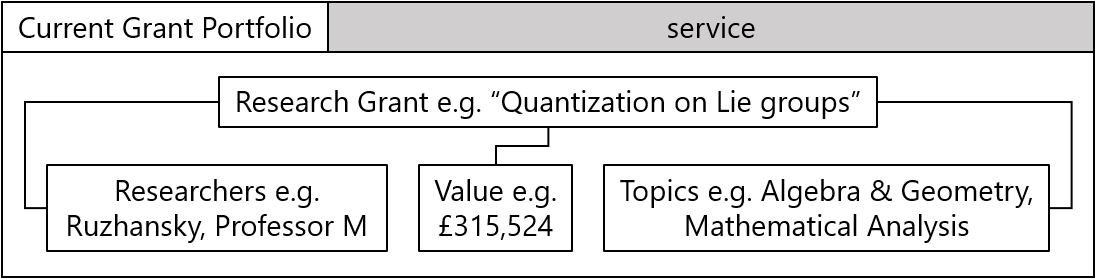
\includegraphics[width=10cm]{portfolios-explained/current_grant_portfolio}
    \caption{Hierarchical structure of the EPSRC Current Grant Portfolio.}
    \label{fig:current_grant_portfolio}
\end{figure}

\begin{figure}[htpb]
    \centering
    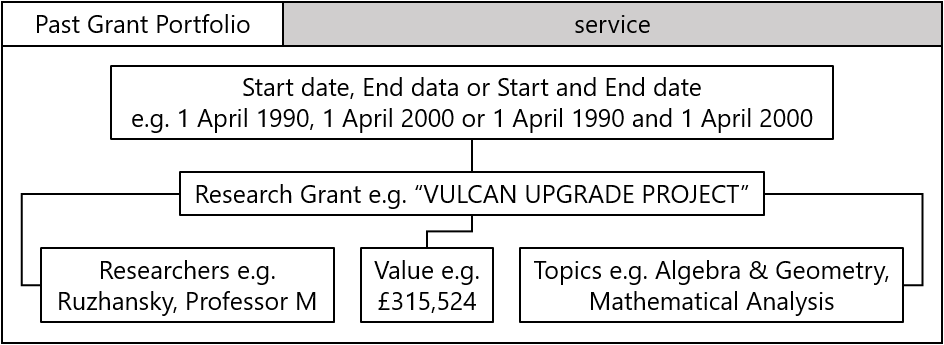
\includegraphics[width=10cm]{portfolios-explained/past_grant_portfolio}
    \caption{Hierarchical Structure of the EPSRC Past Grant Portfolio.}
    \label{fig:past_grant_portfolio}
\end{figure}

Each grant record is stored within a separate web page and contains details about the grant such as \textit{reference}, \textit{investigators (researchers)}, \textit{partners}, \textit{department}, \textit{organisation}, \textit{start} and \textit{end date}, \textit{value} and \textit{topic} and \textit{industrial sector classifications}. Fig. \ref{fig:grant_record} shows an example of a grant record within the \textit{EPSRC Grants on the Web (GoW)} service.

\begin{figure}[htpb]
    \centering
    \fbox{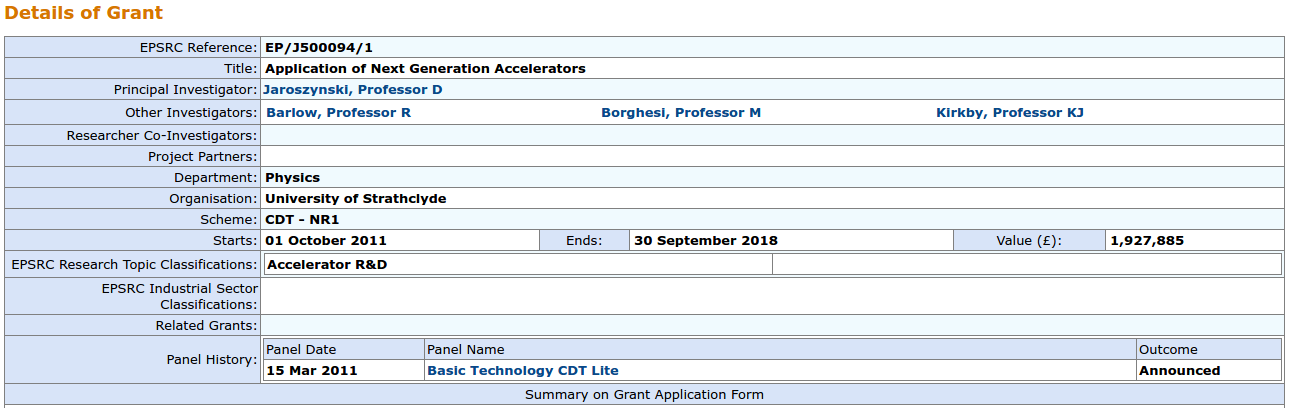
\includegraphics[width=12cm]{epsrc-records/grant_record}}
    \caption{Grant record within the \textit{EPSRC Grants on the Web (GoW)} service.}
    \label{fig:grant_record}
\end{figure}

The researchers within each grant record are linked to separate researcher records. Each researcher record is also stored within a separate web page and contains details about the researcher including \textit{name}, \textit{organisation}, \textit{department}, \textit{current topics} and \textit{grants}. Fig. \ref{fig:researcher_record} shows an example of a researcher record within the \textit{EPSRC Grants on the Web (GoW)} service.

\begin{figure}[htpb]
    \centering
    \fbox{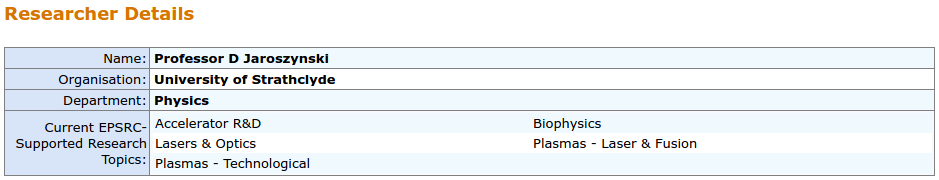
\includegraphics[width=12cm]{epsrc-records/researcher_record}}
    \caption{Researcher record within the \textit{EPSRC Grants on Web (GoW)} service.}
    \label{fig:researcher_record}
\end{figure}

\iffalse
The Current Grant Portfolio within GoW presents data categorised by different research entities such as research area, research topic, theme, industrial sector and so on. This project focuses primarily on research topics, so this entity is used for the following explanation.

The Research Topic page consists of a list of links to different research topics. Within each topic page, a list of links to grants is displayed which related to the topic selected. Each grant page stores information related to the grant such as the researchers working on the grant, the topic classifications of the grant and the value of the grant in British Pounds. Fig. \ref{fig:current_grant_portfolio} illustrates the hierarchical structure of the Current Grant Portfolio.

\begin{figure}[htpb]
    \centering
    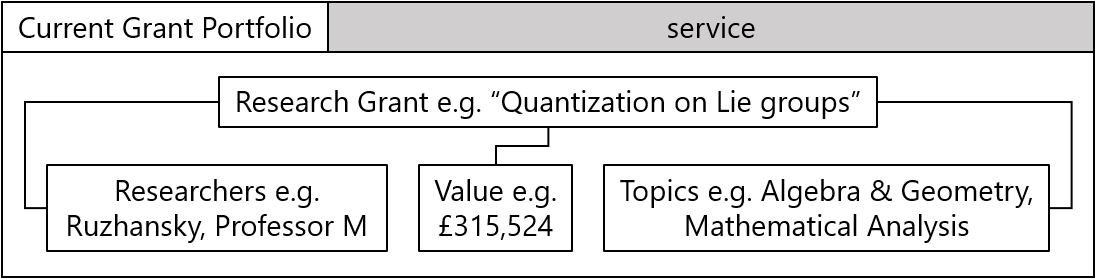
\includegraphics[width=14cm]{portfolios-explained/current_grant_portfolio}
    \caption{Hierarchical structure of the Current Grant Portfolio.}
    \label{fig:current_grant_portfolio}
\end{figure}
\fi

\iffalse
In contrast, the Past Grant Portfolio requires the user to specify a time period and it directly retrieves a list of links to grants based on it. Therefore, the data is only categorised by a time period which represents
either when the grants commenced, completed or commenced and completed. Identically to the Current Grant Portfolio, each grant page stores information including the researchers, topics and value of the grant. Fig. \ref{fig:past_grant_portfolio} illustrates the structure of the Past Grant Portfolio.

\begin{figure}[htpb]
    \centering
    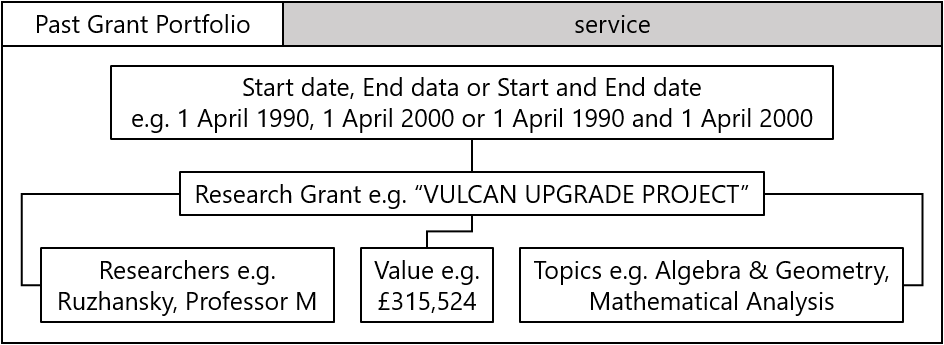
\includegraphics[width=14cm]{portfolios-explained/past_grant_portfolio}
    \caption{Structure of the Past Grant Portfolio.}
    \label{fig:past_grant_portfolio}
\end{figure}
\fi

\iffalse
\subsection{Issues}

For each record, the web scraper has to make a web request, similar to when a user navigates to a web page, and then extract the specified data. For example, to extract data from all current grant records, 3, 175 requests need to be performed. This may not be too problematic, however, for grant data between 2010 and 2000, 18,692 requests are required. Now, that is problematic. Therefore, during the initial process of data extraction, this problem was identified, as the computational time of the past data extraction process was far too lengthy.

Several alternatives were identified as potential solutions to the problem. The scraper could be modified to make asynchronous requests or the physical HTML files could be downloaded and then scraped locally. The latter alternative was chosen, and a script was written in Bash in order to achieve it. This decision was successful and it greatly improved the computational time of the data extraction task.
\fi

\iffalse
\subsection{Process}

In order to extract content from a web page, the page needs to be scraped. This is usually achieved by either using an already built web scraper or by developing a web scraper, which extracts specified data from the underlying tags within the HTML code. In this project, a web scraper was developed using the \textit{requests} and \textit{lxml} Python libraries.

Due to the differences between the Current and Past Grant Portfolios, the data extraction process was also different. All actual data is extracted from either a grant or researcher page. However, to access the grant and researcher pages different series of steps are required depending on whether it is current or past data that is being extracted.

For current data, topic URLs need to be extracted first. Further, the web scraper connects to each topic URL and extracts the grant URLs. Only after the grant URLs are obtained, the web scraper connects to each grant page and begins to extract the actual data. For past data, the process is much simpler as the list of links to grants is supplied directly. This means that the web scraper extracts the grant URLs and then connects to each URLs and starts to extract past grant information. Table \ref{table:data_statistics} presents the number of past and current records within each entity that data was extracted from.

Once extracted, the data is validated and then formatted into a format that allows easy manipulation of it. Finally, it is stored within numerous comma-separated files categorised by content.
\fi

\section{Collection of data from EPSRC}

The previous sections provided an introduction to the data provided by EPSRC, the \textit{Grants on the Web service (GoW)}, the Current and Past Grant Portfolios and the Grant and Researcher records. This project solely uses data collected from the Current and Past Grant Portfolios, and does not use any of the other information provided through the \textit{Grants on the Web (GoW)} service. In terms of the Current and Past Grant Portfolios, this project only makes use of data extracted from grant and researcher records. 

Firstly, data within the following fields of a grant record was extracted:
\textit{EPSRC Reference}, \textit{Principal Investigator}, \textit{Other Investigators}, \textit{Starts}, \textit{Ends} and \textit{EPSRC Research Topic Classifications}. Secondly, data within the \textit{Name} and \textit{Current EPSRC-Supported Research Topics} fields of a researcher record was extracted. 

Furthermore, this project solely extracts the name and current topics from each researcher record. Table \ref{table:grant_researcher_record_numbers} presents the number of current EPSRC grant and researcher records and historical grant records from which data was collected.

Furthermore, this project uses both current and historical data collected from EPSRC, which is organised into two main data sets, while the historical data set is further divided into two sub-data sets as follows:

\begin{itemize}[itemsep=0cm]
    \item \textbf{Current data set}, consisting of current grants (post 2010 start date) and researchers collected on 8 July 2016 
    \item \textbf{Historical data set}, consisting of grant records from two time periods:
    \begin{itemize}[itemsep=0cm]
        \item \textbf{from 1990 to 2000}, consisting of grant records which started and ended between 1 April 1990 and 1 April 2000
        \item \textbf{from 2000 to 2010}, consisting of grant records which started and ended between 1 April 2000 and 1 April 2010
    \end{itemize}
\end{itemize}

\begin{table}[!htbp]
\centering
\caption{Number of current EPSRC grant and researcher records and historical grant records from which data was collected.}
\label{table:grant_researcher_record_numbers}
\begin{tabular}{r|r|r|r}
{} & \multirow{2}{*}{\textbf{Current}}
& \multicolumn{2}{c}{\textbf{Historical}}\\
\cline{3-4}
& {} & \textbf{1990-2000} & \textbf{2000-2010}\\
\hline
\textbf{Number of Grant records}      & {3175} & {17861} & {18692}\\
\textbf{Number of Researcher records} & {5874} & {10820} & {13385}\\
\end{tabular}
\end{table}

The previous section specified that both grant and researcher records are stored as separate web pages within the \textit{Grants on the Web (GoW)} service. In order to extract content from a web page, a technique called \textit{web scraping} is employed. This is usually achieved by either using a third-party web scraper or by developing a web scraper from scratch, which extracts specified data from the underlying tags within the HTML code. In this case, a web scraper was developed using the \textit{requests} and \textit{lxml} Python libraries.

Essentially, the web scraper connects to the URL of each grant and researcher record web page and extracts the text found under specific fields such as \textit{Reference}, \textit{Principal Investigator} and \textit{Other Investigators}, \textit{Value} and \textit{EPSRC Research Topic Classifications}. Once extracted, the data is validated and then comma-delimited and text qualified using quotation marks which preserves its original format and allows easy manipulation of it. Subsequently, it is stored within comma-separated files categorised by content and data set.

\section{Generation of networks from EPSRC data}

In the previous section, the data collection process was explained and documented. The data extracted from the \textit{Grants on the Web (GoW)} service was used to construct several networks of topics and researchers structured as follows:

\begin{enumerate}[itemsep=0cm, label*=\arabic*.]
    
    \item \textbf{Networks of Topics, with nodes representing Topics}
    \begin{enumerate}[itemsep=0cm, label*=\arabic*.]
        \item and edges representing Grants, named \underline{Grants as edges};
            \begin{enumerate}[itemsep=0cm, label*=\arabic*.]
                \item created using the current and historical data sets (1990-2010)
            \end{enumerate}
        \item and edges representing Researchers, named \underline{Researchers as edges};
            \begin{enumerate}[itemsep=0cm, label*=\arabic*.]
                \item constructed using the current data set only\footnote{The Topic (Nodes as Topics, Edges as Researchers) and Researcher network (Nodes as Researchers, Edges as Topics) were created using the Current data set only because Researcher records only consist of a researcher's current topics, and not their historical topics.}
            \end{enumerate}
    \end{enumerate}

    \item \textbf{Networks of Researchers, with nodes representing Researchers}
    \begin{enumerate}[itemsep=0cm, label*=\arabic*.]
        \item and edges representing Grants, named \underline{Grants as edges};
        \begin{enumerate}[itemsep=0cm, label*=\arabic*.]
                \item created using the current and historical data sets (1990-2010)
            \end{enumerate}
        \item and edges representing Topics, named \underline{Topics as edges};
        \begin{enumerate}[itemsep=0cm, label*=\arabic*.]
                \item constructed using the current data set only\footnotemark[1]
        \end{enumerate}
    \end{enumerate}

\end{enumerate}

Node and edge attributes were also formulated and incorporated into the networks. The attribute values "suffered" a normalization process which decreased the scale of the value range. This was followed by extensive experiments which aimed to identify an optimal edge weight and community detection algorithm. Several edge weights (\textit{unweighted}, \textit{weighted by normalized number of projects} and \textit{weighted by normalized value of projects}) and community detection algorithms (\textit{Spinglass}, \textit{Louvain}, \textit{Fast Greedy}) were considered. The optimal solution was chosen based on the modularity score and coherence of the generated topic and researcher clusters.

This section describes how the collected data was used further in the next phase of development including network generation and topic and researcher clustering.

\subsection{Networks of Topics}

The concept of the topic-based network involved two potential ways that the network could be constructed. The topics could be analysed from the perspective of grants as well as researchers. This resulted in the creation of two different networks of topics. In both networks, nodes represent topics. However, edges represent either grants or researchers. For ease of reference, the two networks will be referred to as \textit{Grants as edges} and \textit{Researchers as edges}, respectively.

\subsubsection{Topic network (Grants as edges)}

This network consists of nodes representing topics and edges representing grants. An edge between two nodes means that two topics have a grant in common. Each grant record consists of a \textit{EPSRC Research Topic Classifications} field consisting of research topics that classify the grant. In order to achieve the creation of this network, grants with two or more topics had to considered. For each grant record, an edge was "drawn" between each of the topics. Fig. \ref{fig:topic_a_structure} provides a visual explanation of the network's structure. The network consists of two node and edge attributes, number and value of grants. Furthermore, the node and edge attributes are explained further in the \textit{Node and Edge attributes} section.

\begin{figure}[!htbp]
    \centering
    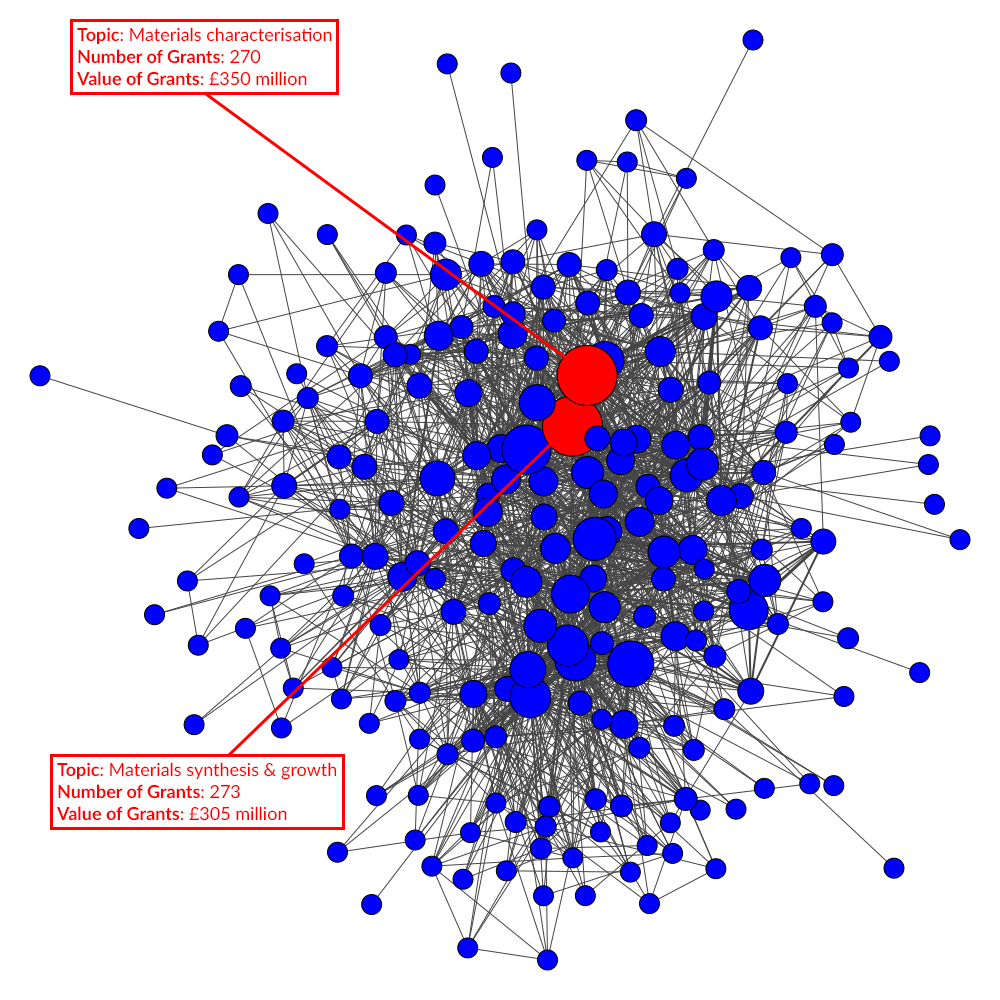
\includegraphics[width=7cm]{networks-explained/topic_network_a}
    \caption{Visual explanation of how the Topic network (Grants as edges) was constructed including the formulated node and edge attributes.}
    \label{fig:topic_a_structure}
\end{figure}

\subsubsection{Topic network (Researchers as edges)}

This network consists of nodes representing topics and edges representing researchers. An edge between two nodes means that two topics have a researcher in common. Each researcher record consists of a \textit{Current EPSRC-Supported Research Topics} field consisting of the researcher's current research topics. In order to achieve the creation of this network, researchers with two or more current topics had to be considered. For each researcher record, an edge was "drawn" between each of the topics. Fig. \ref{fig:topic_b_structure} provides a visual explanation of the network's structure. Furthermore, the network consists of a node and edge attribute, number of researchers. The formulation of node and edge attributes is explained in detail in the \textit{Node and Edge attributes} section.

\begin{figure}[!htbp]
    \centering
    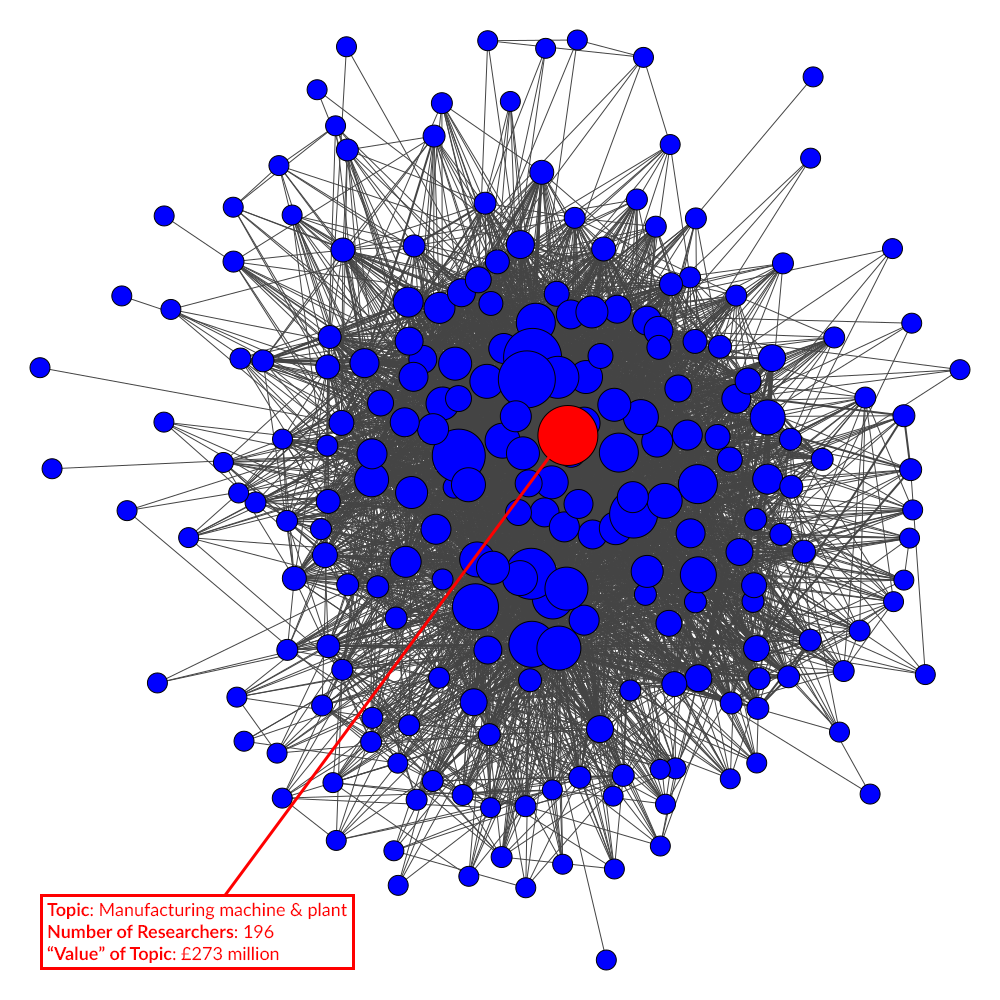
\includegraphics[width=8cm]{networks-explained/topic_network_b}
    \caption{Visual explanation of how the Topic network (Researchers as edges) was constructed including the formulated node and edge attributes.}
    \label{fig:topic_b_structure}
\end{figure}

\subsection{Networks of Researchers}

The concept of the researchers network involved two potential ways that the network could be constructed. The researchers could be analysed from the perspective of grants as well as topics. This resulted in the creation of two different networks of researchers. In both networks, nodes represent researchers. However, edges represent either grants or topics.  For ease of reference, the networks will be referred to as \textit{Grants as edges} and \textit{Topics as edges}, respectively.

\subsubsection{Researcher network (Grants as edges)}

This network consists of nodes representing researchers and edges representing grants. An edge between two nodes means that two researchers have a grant in common. Each grant record consists of the \textit{Principal} and \textit{Other Investigators} fields consisting of researchers collaborating on the grant. In order to achieve the creation of this network, grants with two or more researchers were considered. For each grant record, an edge was "drawn" between each of the researchers. Fig. \ref{fig:researcher_a_structure} provides a visual explanation of the network's structure. Due to the significantly large size of the \textit{Researcher network (Grants as edges)}, the network had to be sampled with the sample consisting of nodes connected by edges with an edge weight of 2 or more. Furthermore, the network consists of two node and edge attributes, number and value of grants. The formulation of node and edge attributes is explained in detail in the \textit{Node and Edge attributes} section.

\begin{figure}[htpb]
    \centering
    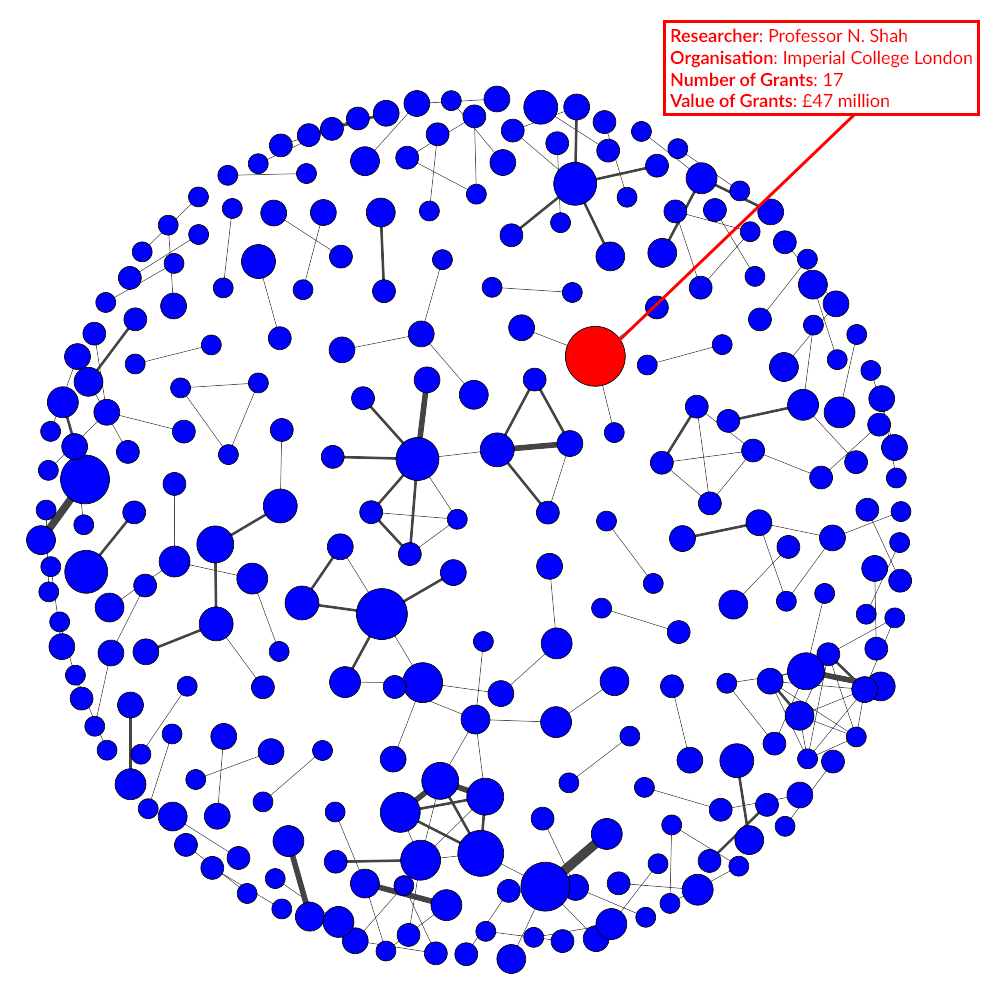
\includegraphics[width=8cm]{networks-explained/researcher_network_b}
    \caption{Visual explanation of how the Researcher network (Grants as edges) was constructed including the formulated node and edge attributes.}
    \label{fig:researcher_a_structure}
\end{figure}

\subsubsection{Researcher network (Topics as edges)}

This network consists of nodes representing researchers and edges representing topics. An edge between two researchers means that two researchers have a topic in common. Each researcher record consists of a \textit{Current EPSRC-Supported Research Topics} field consisting of the researcher's current research topics. In order to achieve the creation of this network, each researcher was compared to all other researchers and if they had at least one topic in common, an edge was "drawn" between the researchers. Fig. \ref{fig:researcher_b_structure} provides a visual explanation of the network's structure. Due to the significantly large size of the \textit{Researcher network (Topics as edges)}, the network had to be sampled with the sample consisting of nodes connected by edges with an edge weight of 5 or more. Furthermore, the network consists of a node and edge attribute, number of topics. The formulation of node and edge attributes is explained in detail in the \textit{Node and Edge attributes} section.

\begin{figure}[htpb]
    \centering
    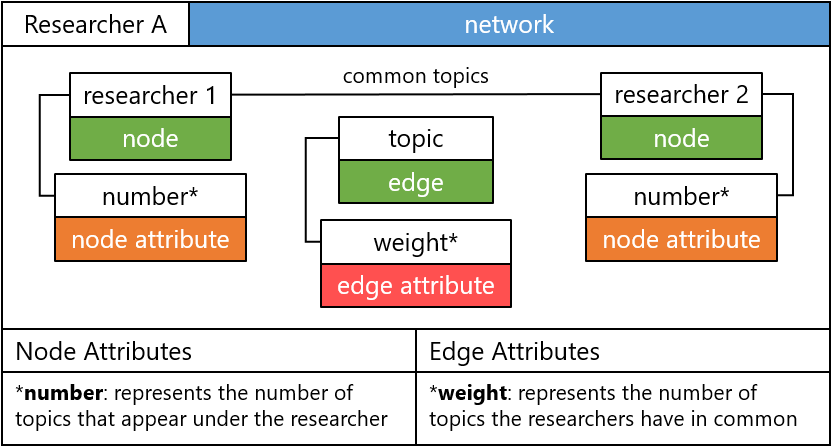
\includegraphics[width=8cm]{networks-explained/researcher_network_a}
    \caption{Visual explanation of how the Researcher network (Topics as edges) was constructed including the formulated node and edge attributes.}
    \label{fig:researcher_b_structure}
\end{figure}

\subsection{The contrast between grants as edges and grant records}

It is essential to point out that there is a clear difference between grants represented by edges and the actual grant records that appear on the \textit{Grants on the Web (GoW)} service. First and foremost, the former is not unique within a network, while the latter is unique within the GoW service. This is because of the way links between topics or researchers were established in a network. For example, if a grant is classified by three topics, each topic is linked to one another by a separate edge, which represents the common grant in question. Therefore, in this case, three edges are created to link the topics which represent the same common grant, meaning that the grant will appear within the network three times. It is also crucial to specify that unlike grants, a network consists of nodes representing unique topics.

This causes issues when questions like the following are posed: \textit{How many grants are in a specific community within a network's community structure?} \textit{What is the value of the grants?} It is important to mention that it is not known which grant is represented by an edge. It is only known that it represents one or more grants depending on the edge weight. If this was known, providing an answer to the above questions becomes significantly easier. In contrast, the answer was achieved through a lengthier process. Furthermore, the edges linking topics within the same community and the edges linking topics in different communities were known. This greatly aided the identification process of both the number and value of grants within communities and between communities.

Firstly, the origin and destination topics of an edge within a network were retrieved. Secondly, during the data collection process, a data structure was created which stored the reference of each grant and the topics that classify it. Next, a check was carried out against all grant records which verified whether both the retrieved origin and destination topics appeared under a grant record. Number and value counters were created to keep track of the cumulative number and value of grants. When the check was true, the reference and value of the grant were added as the key and value to a Python dictionary, in which all keys must be unique. Finally, at the end of the check, the number of grant references was counted and the grant values were summed up. This provided an answer to the questions asked, as the number and value of grants within a community was successfully identified. Additionally, using the same technique, the computation of the number and value of grants between communities and within the entire network was also achieved. The function written in order to achieve this task can be viewed in Code snippet \ref{listing:turn_edges_into_grants} within Appendix \ref{appendix:code}.

\subsection{Formulation of node and edge attributes}

Every network constructed using the data collected from EPSRC consists of at least one node and edge attribute, while others consist of two attributes. Both \textit{Topic} and \textit{Researcher networks (Grants as edges)} consist of a \textit{number} and \textit{value} attribute, while the \textit{Topic (Researchers as edges)} and \textit{Researcher (Topics as edges)} networks only consist of a \textit{number} attribute. Visually, the network attributes control both the size of the node circle and the thickness of the edge line. This section documents the formulation of the node and edge attributes, which allow the analysis and visualisation of the network from two different perspectives.

\subsubsection{Number of grants/topics/researchers}

The number attribute has a number of different contexts, depending on the network. Firstly, in the \textit{Topic} and \textit{Researcher networks (Grants as edges)}, the node number attribute represents the number of grants that contain a topic or researcher. In the same networks, the edge number attribute represents the number of grants two topics or researchers have in common, meaning they are both contained within the same grant record. Secondly, in the \textit{Topic network (Researchers as edges)}, the node number attribute represents the number of researchers that contain the topic, while the edge number attribute represents the number of researchers two topics have in common, meaning they are both contained within the same researcher record. Thirdly, in the \textit{Researcher network (Topics as edges)}, the node number attribute represents the number of topics a researcher currently has, while the edge number attribute represents the number of topics two researchers have in common.

\subsubsection{Value of grants}

Similarly, the value attribute also has a number of different contexts, depending on the network. Firstly, networks that are not based on grant data do not contain of the value attribute. Secondly, in the \textit{Topic} and \textit{Researcher network (Grants as Edges)}, the node value attribute represents the value of a topic or researcher. This represents the value of the grants that contain that specific topic or researcher. In the same network, the edge value attribute represents the value of the grants that two topics or researcher have in common, meaning they are both contained within the same researcher record.

\subsection{Normalization of node and edge attribute values}

The numerical values used as the node and edge attributes, especially the value attribute, represent significantly large numbers which cause issues in terms of development, analysis and visualisation. To accommodate this, the values underwent a normalization process which scaled the value range down. The function written in order to achieve this task can be viewed in Code snippet \ref{listing:norm_vals} within Appendix \ref{appendix:code}, while the formula used to normalize the values is presented below:

\begin{equation}
    (val - old\_min) \times new\_range / old\_range) + new\_min)
\end{equation}
where:
\begin{itemize}[itemsep=0cm]
    \item \textit{val} is the value being normalized
    \item \textit{old\_min} is the minimum of the initial value range
    \item \textit{new\_range} is the new range values will be normalized to
    \item \textit{old\_max} is the maximum of the initial value range
    \item \textit{new\_min} is the minimum of the new value range
\end{itemize}

\section{Comparison of edge weights and community detection algorithms}

In the previous section, the process carried out to normalize the values used as node and edge attributes was described. This section details the experiments carried in order to identify the most coherent division of the topic and researcher networks into topic and researcher clusters.

Several experiments were carried seeking to identify an optimal edge weight and community detection algorithm that produced the most rational clustering results. In order to ensure a consistent analysis, the experiments were solely carried out on the \textit{Topic} and \textit{Researcher network (Grants as edges)}. The results of the experiments on this network were applied to all the other networks.

Eight different community detection algorithms were considered including \textit{Louvain}, \textit{Spinglass} and \textit{Fast Greedy}. The \textit{Topic network (Grants as edges)} consists of two node and edge attributes, number and value of grants. The values of both attributes are significantly large and therefore they were normalized for development, analysis and visualisation purposes. In total, three different "candidates" of interpreting the edge weight were considered: \textit{unweighted}, \textit{weighted by normalized number of grants} and \textit{weighted by normalized value of grants}.

Furthermore, the eight community detection algorithms were applied to each network using each of the three edge weight interpretations, while the results of the experiments underwent a multi-phase comparative analysis, documented in the next section.

\section{Identification of an optimal edge weight and community detection algorithm}

The experimental stage consisted of a number phases. In the first phase, a number of community detection algorithms were applied to the network using each of the edge weight interpretations. The resulting modularity scores and number of generated communities were compared across all edge weight and community detection algorithm candidates. Most community detection algorithms make use of the edge weight attribute in the clustering process, which meant that the \textit{unweighted} edge weight interpretation had a low-performance and was excluded from the tests in the first phase. Furthermore, a number of community detection algorithms such as \textit{Label Propagation}, \textit{Leading Eigenvector} and \textit{Edge Betweenness} were also excluded due to low performance results. In contrast, the \textit{Louvain}, \textit{Spinglass} and \textit{Fast Greedy} algorithms remained to be tested further.

During the second phase, the number of topics within each community was compared across all candidates, and it was decided that all remaining edge weight interpretations and community detection algorithms would proceed to the final testing phase. In the third phase and the final phase, each community of topics identified using each one of the edge weight interpretations and community detection algorithms were compared to each other based on coherence and balance. Finally, it was concluded that the clustering produced by the \textit{normalized number of grants/topics/researchers} edge weight interpretation and the \textit{Louvain} community detection algorithm was the most reasonable and the one that would be employed throughout the rest of the analysis.

\section{Clustering of Topics and Researchers}

As revealed in the previous section, the \textit{Louvain} community detection algorithm performed the best when applied to a network in which the weight of an edge represents the \textit{normalized number of grants, topics or researchers}. Following this discovery, the identified combination of edge weight and community detection algorithm was considered the optimal solution.

Furthermore, the solution was applied to each network in order to identify its underlying community structure. This resulted in a number of communities also known as clusters or groups, consisting of topics or researchers. Each topic or researcher was assigned to exactly one cluster. Certain identified communities can be quite broad in terms of the representation of research areas, especially if the network consists of a large number of nodes. In order to achieve a more specific clustering, the community detection algorithm was applied to each previously identified community in order to discover its sub-communities which form each community's underlying community structure.

Moreover, the topic and researcher clustering was documented in a Microsoft Excel spreadsheet. The number and value of grant records in each community was also documented and calculated. This was followed by the creation of word cloud representations of the communities and sub-communities identified within the \textit{Topic network (Grants as edges)}, using Wordle. Each community and sub-community was illustrated from three different perspectives: \textit{word frequency}, \textit{number of grants} and \textit{value of grants}.

\section{Evaluation of Topic and Researcher clusters}

Once the topic and researcher clusters were identified and defined, they underwent an evaluation stage which determined how strong the links between nodes in the same clusters are compared to links that connect nodes that are in different clusters. This was achieved by calculating the Dice and Jaccard similarity of nodes within the same and different clusters.

Firstly, the origin and destination nodes of each edge in the network were identified. This forms a pair of nodes as follows: origin node, destination node. Certain edges connect nodes that are in the same cluster, while others link nodes that are in different clusters. Therefore, some node pairs represent nodes from the same cluster, while others represent nodes from different clusters. Secondly, the Dice and Jaccard similarity between each node pair was calculated. Theoretically, a pair of nodes from the same cluster should be more similar than a pair of nodes from different clusters. The evaluation phase helped to determine whether in reality this is also true. Finally, in order to obtain an overall perspective of the similarity of nodes within and between clusters, the average Dice and Jaccard similarity was calculated.

\section{Tools used in this project}

During this study, several tools were employed in order to accomplish various development and analysis activities. This section describes the tools and comments on their use throughout the project.

\subsection{JetBrains PyCharm used for programming}

JetBrains PyCharm \cite{jetbrains_pycharm} is an Integrated Development Environment (IDE) for programming in Python. It also provides support for writing code in Bash. It was used to write the development code in primarily Python but also in Bash.

\subsection{Microsoft Excel used for data storage}

Microsoft Excel \cite{microsoft_excel} is a spreadsheet software featuring calculation, graphing tools, pivot tables, and macro programming support in Visual Basic. It was used to explore, filter and validate the collected data.

\subsection{iGraph used for network analysis and visualisation}

iGraph \cite{csardi2006igraph} is a library collection for creating and manipulating graphs and analyzing networks. This tool was used to compute network properties, apply community detection algorithms, and produce visualisations of the networks created.

\subsection{NetworkX used for visualising adjacency matrices}

NetworkX \cite{networkx} is a package for the creation, manipulation, and study of the structure, dynamics, and functions of complex networks in Python. It was used to visualise adjacency matrices.

\subsection{Wordle used for creating word cloud visualisations}

Wordle \cite{wordle} is a tool for visualising text as word clouds. By default, it computes each word's frequency and displays the more frequent words in a larger font than less frequent ones. Additionally, Wordle's advanced mode allows keeping words together, specifying a weight which control the font size as well as specifying a colour for each word. It was to create word cloud representations of topic clusters using several attributes to control font size and colour.

\subsection{Adobe Photoshop used for image editing}

Adobe Photoshop \cite{adobe_photoshop} is a graphics editor developed by Adobe Systems. It was used for image editing as well as turning network plots produced using iGraph into complete network visualisations.
\chapter{Results}
\label{chapterlabel5}

\blindtext
\chapter{\textsc{Analysis of Results}}
\label{chapterlabel6}

\section{Topic clustering}

\section{Researcher clustering}
\addcontentsline{toc}{chapter}{Appendices}

% The \appendix command resets the chapter counter, and changes the chapter numbering scheme to capital letters.
%\chapter{Appendices}
\appendix
\chapter{An Appendix About Stuff}
\label{appendixlabel1}

\chapter{Another Appendix About Things}
\label{appendixlabel2}

\chapter{Colophon}
\label{appendixlabel3}
\textit{This is a description of the tools you used to make your thesis. It helps people make future documents, reminds you, and looks good.}

\textit{(example)} This document was set in the Times Roman typeface using \LaTeX\ and Bib\TeX , composed with a text editor. 
 % description of document, e.g. type faces, TeX used, TeXmaker, packages and things used for figures. Like a computational details section.
% e.g. http://tex.stackexchange.com/questions/63468/what-is-best-way-to-mention-that-a-document-has-been-typeset-with-tex#63503

% Side note:
%http://tex.stackexchange.com/questions/1319/showcase-of-beautiful-typography-done-in-tex-friends
% You could separate these out into different files if you have
%  particularly large appendices.

% This line manually adds the Bibliography to the table of contents.
% The fact that \include is the last thing before this ensures that it
% is on a clear page, and adding it like this means that it doesn't
% get a chapter or appendix number.
\addcontentsline{toc}{chapter}{Bibliography}

% Actually generates your bibliography.
\bibliography{bibliography/bibliography}

% All done. \o/
\end{document}
